\frame{
  \frametitle{Los tres estados} 
  Git tiene tres estados principales, que tus archivos pueden poseer:
  \begin{itemize}
  \item Commited: Guardado sin peligro en tu repositorio.
  \item Modified: El archivo tiene cambios, pero no se ha agregado.
  \item Staged: Agregado, pero no se ha hecho el commit al repositorio.
  \end{itemize}

  Esto nos conduce tambi\'en a las tres principales secciones de Git: 
       
\begin{figure}[t]
    \centering
    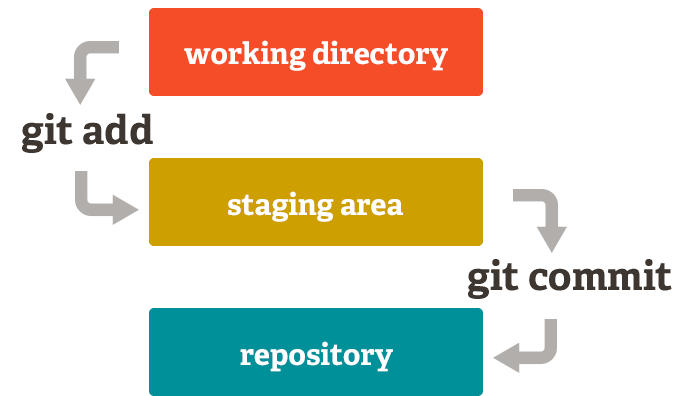
\includegraphics[width=0.5\textwidth]{Images/5}
\end{figure}
  }    
